%==============================================================
%  From Neural Networks to LLMs -- A Visual Intuition
%  A Beamer presentation for technical data people with no
%  deep-learning background. Styled after the 3Blue1Brown
%  deep learning playlist: pictures first, formulas last.
%
%  Compile with:  pdflatex nn-to-llm.tex   (run twice)
%  Present in your PDF viewer's fullscreen / presentation mode.
%==============================================================
\documentclass[aspectratio=169,11pt]{beamer}

\usetheme{Madrid}
\usecolortheme{whale}
\setbeamertemplate{navigation symbols}{}

\usepackage[T1]{fontenc}
\usepackage[utf8]{inputenc}
\usepackage{lmodern}
\usepackage{amsmath}
\usepackage{amssymb}
\usepackage{tikz}
\usetikzlibrary{arrows.meta,positioning,shapes.geometric,calc,fit,backgrounds}

%---------------- colour palette -------------------------------
\definecolor{nnblue}{RGB}{31,84,142}
\definecolor{nnlight}{RGB}{225,236,247}
\definecolor{nnorange}{RGB}{214,124,29}
\definecolor{nnsand}{RGB}{252,240,222}
\definecolor{nngreen}{RGB}{40,124,86}
\definecolor{nnmint}{RGB}{224,240,232}
\definecolor{nnred}{RGB}{176,58,58}
\definecolor{nngray}{RGB}{100,100,100}

\setbeamercolor{structure}{fg=nnblue}
\setbeamercolor{palette primary}{bg=nnblue,fg=white}
\setbeamercolor{title}{bg=nnblue,fg=white}
\setbeamercolor{frametitle}{bg=nnblue,fg=white}
\setbeamercolor{block title}{bg=nnblue,fg=white}
\setbeamercolor{block body}{bg=nnlight,fg=black}
\setbeamercolor{block title alerted}{bg=nnred,fg=white}
\setbeamercolor{block title example}{bg=nngreen,fg=white}
\setbeamercolor{block body example}{bg=nnmint,fg=black}
\setbeamerfont{frametitle}{series=\bfseries}
\setbeamerfont{title}{series=\bfseries}
\setbeamertemplate{itemize item}{\color{nnblue}$\blacktriangleright$}
\setbeamertemplate{itemize subitem}{\color{nnorange}$\bullet$}

% compact footline: author | title | frame number
\setbeamertemplate{footline}{%
  \hbox{%
  \begin{beamercolorbox}[wd=.32\paperwidth,ht=2.4ex,dp=1.2ex,left,leftskip=1em]{author in head/foot}%
    \usebeamerfont{author in head/foot}\insertshortauthor
  \end{beamercolorbox}%
  \begin{beamercolorbox}[wd=.53\paperwidth,ht=2.4ex,dp=1.2ex,center]{title in head/foot}%
    \usebeamerfont{title in head/foot}\insertshorttitle
  \end{beamercolorbox}%
  \begin{beamercolorbox}[wd=.15\paperwidth,ht=2.4ex,dp=1.2ex,right,rightskip=1em]{date in head/foot}%
    \usebeamerfont{date in head/foot}\insertframenumber\,/\,\inserttotalframenumber
  \end{beamercolorbox}}%
}

%---------------- reusable tikz styles -------------------------
\tikzset{
  box/.style   = {rounded corners=3pt, draw=nnblue, thick, fill=nnlight,
                  align=center, inner sep=5pt, minimum height=0.85cm, font=\small},
  obox/.style  = {box, draw=nnorange, fill=nnsand},
  gbox/.style  = {box, draw=nngreen, fill=nnmint},
  rbox/.style  = {box, draw=nnred, fill=red!8},
  tok/.style   = {rounded corners=2pt, draw=nngray, fill=white,
                  font=\small, inner sep=4pt, minimum height=0.7cm},
  neuron/.style= {circle, draw=nnblue, fill=nnlight, inner sep=0pt,
                  minimum size=5.5mm},
  ar/.style    = {-{Stealth[length=2.4mm]}, thick, draw=nngray},
  thinar/.style= {-{Stealth[length=1.8mm]}, draw=nngray, line width=0.5pt},
  lbl/.style   = {font=\scriptsize\itshape, text=nngray},
}

% ---- overlay-aware TikZ ---------------------------------------
% "visible on=<2->" hides a node/path on other slides WITHOUT
% removing it, so nothing shifts as the diagram builds up.
\tikzset{
  invisible/.style   = {opacity=0},
  visible on/.style  = {alt={#1{}{invisible}}},
  alt/.code args     = {<#1>#2#3}{%
    \alt<#1>{\pgfkeysalso{#2}}{\pgfkeysalso{#3}}%
  },
}

%---------------- title data -----------------------------------
\title[Neural Networks to LLMs]{From Neural Networks to LLMs}
\subtitle{A Visual Intuition}
\author[NN $\rightarrow$ LLM]{Adham}
\institute{}
\date{\today}

\begin{document}

%============================================================== 1
\begin{frame}[plain]
  \titlepage
  \begin{center}
    \small\color{nngray}
    No prior knowledge of deep learning assumed --- we start from pixels.
  \end{center}
\end{frame}

%============================================================== 2
\begin{frame}{The big picture}
  \begin{block}{The claim}
    Everything from recognising a handwritten digit to writing an essay
    runs on \textbf{one} idea, repeated and scaled.
  \end{block}
  \medskip
  \begin{center}
  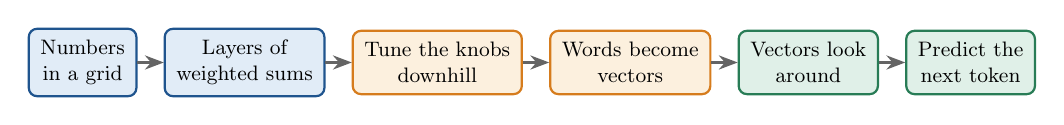
\begin{tikzpicture}[node distance=4mm, scale=0.84, transform shape]
    \node[box, visible on=<2->]                 (a) {Numbers\\in a grid};
    \node[box, right=of a, visible on=<3->]     (b) {Layers of\\weighted sums};
    \node[obox, right=of b, visible on=<4->]    (c) {Tune the knobs\\downhill};
    \node[obox, right=of c, visible on=<5->]    (d) {Words become\\vectors};
    \node[gbox, right=of d, visible on=<6->]    (e) {Vectors look\\around};
    \node[gbox, right=of e, visible on=<7->]    (f) {Predict the\\next token};
    \draw[ar, visible on=<3->] (a) -- (b);
    \draw[ar, visible on=<4->] (b) -- (c);
    \draw[ar, visible on=<5->] (c) -- (d);
    \draw[ar, visible on=<6->] (d) -- (e);
    \draw[ar, visible on=<7->] (e) -- (f);
  \end{tikzpicture}
  \end{center}
  \medskip
  \begin{itemize}
    \item<8-> You already think in tables, joins and pipelines
    \item<8-> Today: think in \textbf{grids, landscapes and directions}
  \end{itemize}
  \medskip
  \uncover<9->{\centering\small\color{nngray}
  There is no step where magic gets added.}
\end{frame}

%============================================================== 3
\begin{frame}{What is a neural network?}
  \begin{columns}[T,onlytextwidth]
    \begin{column}{0.46\textwidth}
      \small
      The classic example: recognise a handwritten digit.
      \begin{itemize}
        \item<2-> A $28\times28$ image is just \textbf{784 numbers}
        \item<3-> A \alert{neuron} is nothing but a thing that
              \textbf{holds a number}
        \item<4-> Each neuron takes a \textbf{weighted sum} of the whole
              previous layer
        \item<5-> \textbf{Weights} $=$ strength of each connection
        \item<5-> \textbf{Bias} $=$ how high the sum must climb before this
              neuron fires
      \end{itemize}
      \uncover<6->{%
      \begin{block}{The whole network, in one line}
        \centering $a^{(n+1)} = \sigma\!\left(W a^{(n)} + b\right)$
      \end{block}}
    \end{column}
    \begin{column}{0.50\textwidth}
      \centering
      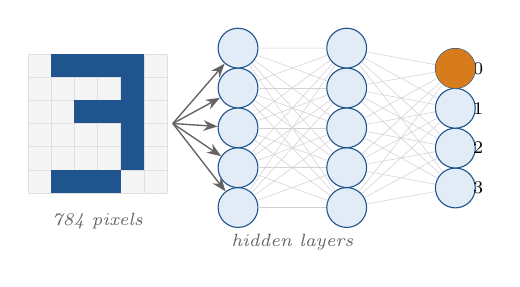
\begin{tikzpicture}[scale=0.92, transform shape]
        % --- pixel grid ---
        \foreach \x in {0,...,5}{
          \foreach \y in {0,...,5}{
            \draw[gray!25, fill=gray!8, line width=0.2pt]
              (\x*0.32,\y*0.32) rectangle (\x*0.32+0.32,\y*0.32+0.32);
          }
        }
        \foreach \x/\y in {1/5,2/5,3/5,4/5, 4/4, 2/3,3/3,4/3, 4/2, 4/1,
                           1/0,2/0,3/0}{
          \fill[nnblue] (\x*0.32,\y*0.32) rectangle (\x*0.32+0.32,\y*0.32+0.32);
        }
        \node[lbl, below] at (0.96,-0.15) {784 pixels};

        % --- layers ---
        \foreach \i in {1,...,5}{
          \node[neuron, visible on=<3->] (a\i) at (2.9, \i*0.55-0.75) {};
          \node[neuron, visible on=<3->] (b\i) at (4.4, \i*0.55-0.75) {};
        }
        \foreach \i/\d in {1/3,2/2,3/1,4/0}{
          \node[neuron, visible on=<3->] (c\i) at (5.9, \i*0.55-0.48) {};
          \node[font=\scriptsize, right=1.2mm, visible on=<3->] at (c\i) {\d};
        }
        \fill[nnorange, visible on=<3->] (5.9, 4*0.55-0.48) circle (2.75mm);

        % --- connections ---
        \foreach \i in {1,...,5}{
          \draw[thinar, visible on=<4->] (2.0, 0.96) -- (a\i);
          \foreach \j in {1,...,5}{
            \draw[gray!35, line width=0.2pt, visible on=<4->] (a\i) -- (b\j);
          }
          \foreach \j in {1,...,4}{
            \draw[gray!35, line width=0.2pt, visible on=<4->] (b\i) -- (c\j);
          }
        }
        \node[lbl, below] at (3.65,-0.45) {hidden layers};
      \end{tikzpicture}

      \smallskip
      \small\color{nngray}
      \uncover<5->{Brightness flows left to right. The brightest output wins.}
    \end{column}
  \end{columns}
\end{frame}

%============================================================== 4
\begin{frame}{How it learns: walking downhill}
  \begin{columns}[T,onlytextwidth]
    \begin{column}{0.47\textwidth}
      \small
      That digit network has \textbf{13{,}002} knobs --- nobody sets them by
      hand.
      \begin{itemize}
        \item<2-> Start with \textbf{random} knobs: the output is garbage
        \item<3-> The \alert{cost function} scores how wrong you are ---
              \textbf{one number}, over thousands of examples
        \item<4-> Picture it as \textbf{altitude} over a landscape of every
              possible knob setting
        \item<5-> Learning $=$ ask ``which way is \textbf{downhill}?'', then
              step
      \end{itemize}
      \uncover<6->{%
      \begin{exampleblock}{Gradient descent}
        The \textbf{gradient} points uphill. Go the other way, a few million
        times.
      \end{exampleblock}}
    \end{column}
    \begin{column}{0.49\textwidth}
      \centering
      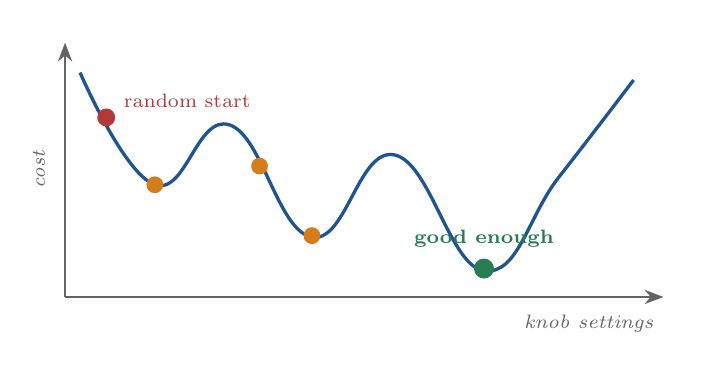
\begin{tikzpicture}[scale=0.95]
        \path[clip] (-0.5,-0.7) rectangle (8.3,3.6);
        \draw[ar] (0,0) -- (8.0,0) node[lbl, below left=1mm and 0mm] {knob settings};
        \draw[ar] (0,0) -- (0,3.4);
        \node[lbl, rotate=90] at (-0.35,1.7) {cost};

        \draw[very thick, nnblue] plot[smooth, tension=0.75] coordinates
          {(0.2,3.0) (1.2,1.5) (2.2,2.3) (3.3,0.8) (4.4,1.9) (5.6,0.35)
           (6.6,1.6) (7.6,2.9)};

        \fill[nnred, visible on=<2->]   (0.55,2.4) circle (3.4pt);
        \node[font=\scriptsize, text=nnred, above right=0mm and 1mm,
              visible on=<2->] at (0.55,2.4) {random start};

        \fill[nnorange, visible on=<3->] (1.2,1.5) circle (3.2pt);
        \fill[nnorange, visible on=<4->] (2.6,1.75) circle (3.2pt);
        \fill[nnorange, visible on=<5->] (3.3,0.82) circle (3.2pt);
        \fill[nngreen,  visible on=<6->] (5.6,0.38) circle (3.8pt);
        \node[font=\scriptsize\bfseries, text=nngreen, above=1.5mm,
              visible on=<6->] at (5.6,0.38) {good enough};
      \end{tikzpicture}

      \smallskip
      \small\color{nngray}
      \uncover<6->{Real landscapes have \textbf{millions} of dimensions ---
      but the move is exactly this: step downhill.}
    \end{column}
  \end{columns}
\end{frame}

%============================================================== 5
\begin{frame}{Words as vectors}
  \begin{block}{The problem}
    Matrix multiplication does not accept the word ``king''. Every input must
    become numbers.
  \end{block}
  \medskip
  \begin{columns}[T,onlytextwidth]
    \begin{column}{0.44\textwidth}
      \small
      \begin{itemize}
        \item<2-> Give every word an \alert{embedding}: a point in a space of a
              few thousand dimensions
        \item<3-> \textbf{Nearby} points $=$ related meanings
        \item<4-> \textbf{Directions} carry meaning too --- one direction
              encodes gender, another plurality, another royalty
      \end{itemize}
      \medskip
      \uncover<5->{%
      \begin{exampleblock}{The famous one}
        \centering
        $\vec{\text{king}} - \vec{\text{man}} + \vec{\text{woman}}
         \;\approx\; \vec{\text{queen}}$
      \end{exampleblock}}
    \end{column}
    \begin{column}{0.52\textwidth}
      \centering
      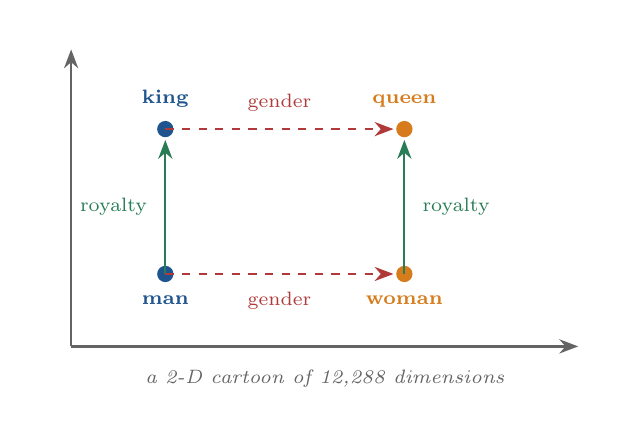
\begin{tikzpicture}[scale=0.92]
        \path[clip] (-0.6,-0.7) rectangle (7.4,4.4);
        \draw[ar] (0,0) -- (7.0,0);
        \draw[ar] (0,0) -- (0,4.1);
        \node[lbl] at (3.5,-0.45) {a 2-D cartoon of 12{,}288 dimensions};

        \fill[nnblue, visible on=<2->] (1.3,1.0) circle (3.2pt);
        \node[font=\scriptsize\bfseries, text=nnblue, below=1.5mm,
              visible on=<2->] at (1.3,1.0) {man};
        \fill[nnblue, visible on=<2->] (1.3,3.0) circle (3.2pt);
        \node[font=\scriptsize\bfseries, text=nnblue, above=1.5mm,
              visible on=<2->] at (1.3,3.0) {king};
        \fill[nnorange, visible on=<2->] (4.6,1.0) circle (3.2pt);
        \node[font=\scriptsize\bfseries, text=nnorange, below=1.5mm,
              visible on=<2->] at (4.6,1.0) {woman};
        \fill[nnorange, visible on=<2->] (4.6,3.0) circle (3.2pt);
        \node[font=\scriptsize\bfseries, text=nnorange, above=1.5mm,
              visible on=<2->] at (4.6,3.0) {queen};

        \draw[ar, draw=nngreen, thick, visible on=<4->] (1.3,1.0) -- (1.3,2.85)
          node[midway, left=1mm, font=\scriptsize, text=nngreen] {royalty};
        \draw[ar, draw=nngreen, thick, visible on=<4->] (4.6,1.0) -- (4.6,2.85)
          node[midway, right=1mm, font=\scriptsize, text=nngreen] {royalty};
        \draw[ar, draw=nnred, thick, dashed, visible on=<5->] (1.3,1.0) -- (4.45,1.0)
          node[midway, below=1mm, font=\scriptsize, text=nnred] {gender};
        \draw[ar, draw=nnred, thick, dashed, visible on=<5->] (1.3,3.0) -- (4.45,3.0)
          node[midway, above=1mm, font=\scriptsize, text=nnred] {gender};
      \end{tikzpicture}

      \smallskip
      \small\color{nngray}
      \uncover<5->{Same step, same direction --- meaning became \textbf{geometry}.}
    \end{column}
  \end{columns}
\end{frame}

%============================================================== 6
\begin{frame}{The context problem}
  Before 2017, text models read \textbf{strictly left to right}, one word at a
  time, carrying a single fixed-size memory.
  \medskip
  \begin{center}
  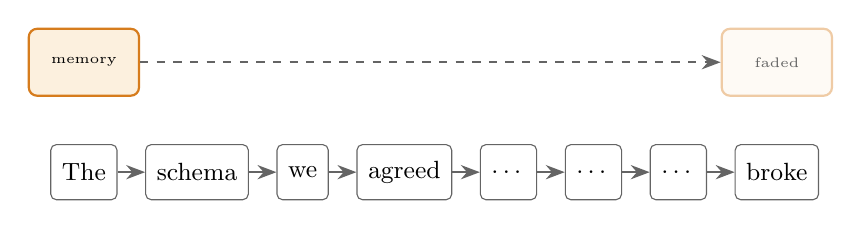
\begin{tikzpicture}[node distance=3.5mm]
    \node[tok] (w1) {The};
    \node[tok, right=of w1] (w2) {schema};
    \node[tok, right=of w2] (w3) {we};
    \node[tok, right=of w3] (w4) {agreed};
    \node[tok, right=of w4] (w5) {\dots};
    \node[tok, right=of w5] (w6) {\dots};
    \node[tok, right=of w6] (w7) {\dots};
    \node[tok, right=of w7] (w8) {broke};
    \foreach \a/\b in {w1/w2,w2/w3,w3/w4,w4/w5,w5/w6,w6/w7,w7/w8}{
      \draw[ar, visible on=<2->] (\a) -- (\b);
    }
    \node[obox, above=6mm of w1, minimum width=1.4cm, visible on=<3->] (m1)
      {\tiny memory};
    \node[obox, above=6mm of w8, minimum width=1.4cm, fill=nnsand!30,
          draw=nnorange!40, visible on=<3->] (m8) {\tiny \color{nngray}faded};
    \draw[ar, dashed, visible on=<3->] (m1) -- (m8);
  \end{tikzpicture}
  \end{center}
  \medskip
  \begin{columns}[T,onlytextwidth]
    \begin{column}{0.478\textwidth}
      \begin{alertblock}<4->{Two hard limits}
        \begin{itemize}
          \item By word 200, word 2 has \textbf{blurred away}
          \item Word $n$ waits for word $n-1$: \textbf{no parallelism}
        \end{itemize}
      \end{alertblock}
    \end{column}
    \begin{column}{0.478\textwidth}
      \begin{block}<5->{What was missing}
        A way for \emph{any} word to reach \emph{any} other word ---
        \textbf{directly}, and \textbf{all at once}.
      \end{block}
    \end{column}
  \end{columns}
\end{frame}

%============================================================== 7
\begin{frame}{Attention: letting vectors look around}
  \begin{columns}[T,onlytextwidth]
    \begin{column}{0.45\textwidth}
      \small
      A word's embedding starts out \textbf{generic} --- the dictionary
      entry, with every meaning blurred together.
      \begin{itemize}
        \item<2-> \alert{Attention} lets each vector \textbf{ask a question} of
              every other word: ``any adjectives near me? any river talk?''
        \item<3-> Words that answer well \textbf{send back} a piece of their
              meaning
        \item<4-> The vector \textbf{moves} --- it now means this word
              \emph{in this sentence}
      \end{itemize}
      \medskip
      \uncover<5->{%
      \begin{exampleblock}{Two banks}
        \small
        ``sat on the river \textbf{bank}'' $\rightarrow$ mud and water\\[2pt]
        ``wired it to the \textbf{bank}'' $\rightarrow$ money and vaults
      \end{exampleblock}}
    \end{column}
    \begin{column}{0.51\textwidth}
      \centering
      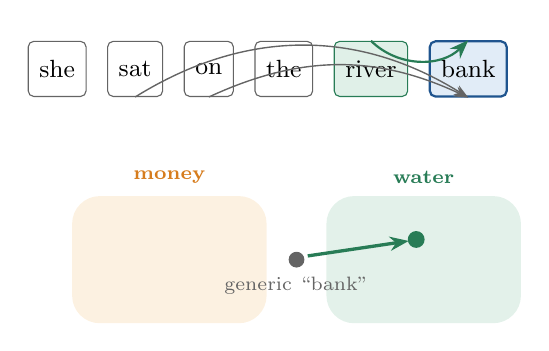
\begin{tikzpicture}[node distance=2.6mm, scale=0.95]
        \node[tok] (t1) {she};
        \node[tok, right=of t1] (t2) {sat};
        \node[tok, right=of t2] (t3) {on};
        \node[tok, right=of t3] (t4) {the};
        \node[tok, right=of t4, fill=nnmint, draw=nngreen] (t5) {river};
        \node[tok, right=of t5, fill=nnlight, draw=nnblue, thick] (t6) {bank};

        \draw[ar, draw=nngreen, thick, visible on=<3->]
          (t5.north) to[bend right=45] (t6.north);
        \draw[thinar, visible on=<3->] (t2.south) to[bend left=32] (t6.south);
        \draw[thinar, visible on=<3->] (t3.south) to[bend left=25] (t6.south);

        % meaning map below
        \begin{scope}[yshift=-3.4cm, xshift=0.2cm]
          \begin{scope}[on background layer]
            \fill[nnsand, rounded corners=10pt, opacity=0.9, visible on=<4->]
                 (0,0) rectangle (2.6,1.7);
            \fill[nnmint, rounded corners=10pt, opacity=0.9, visible on=<4->]
                 (3.4,0) rectangle (6.0,1.7);
          \end{scope}
          \node[font=\scriptsize\bfseries, text=nnorange, visible on=<4->]
               at (1.3,1.95) {money};
          \node[font=\scriptsize\bfseries, text=nngreen, visible on=<4->]
               at (4.7,1.95) {water};

          \fill[nngray, visible on=<4->] (3.0,0.85) circle (3pt);
          \node[font=\scriptsize, below=1mm, text=nngray, visible on=<4->]
               at (3.0,0.85) {generic ``bank''};
          \draw[ar, draw=nngreen, very thick, visible on=<5->]
               (3.15,0.9) -- (4.5,1.1);
          \fill[nngreen, visible on=<5->] (4.6,1.12) circle (3.2pt);
        \end{scope}
      \end{tikzpicture}

      \vspace{2.2cm}
      \small\color{nngray}
      \uncover<6->{Every word does this, for every other word,
      \textbf{in parallel}. That is the Transformer.}
    \end{column}
  \end{columns}
\end{frame}

%============================================================== 8
\begin{frame}{So what makes it ``large''?}
  \begin{block}{Nothing new is invented at the top}
    Same neurons. Same downhill walk. Same attention. Just \textbf{more}.
  \end{block}
  \medskip
  \begin{columns}[T,onlytextwidth]
    \begin{column}{0.478\textwidth}
      \begin{block}{The digit network}
        \small
        \begin{itemize}
          \item $\sim$13{,}000 knobs
          \item Sees $28\times28$ pixels
          \item Trained on 60{,}000 images
          \item Minutes on a laptop
        \end{itemize}
      \end{block}
    \end{column}
    \begin{column}{0.478\textwidth}
      \begin{exampleblock}<2->{A modern LLM}
        \small
        \begin{itemize}
          \item Hundreds of \textbf{billions} of knobs
          \item Context window of a small \textbf{library}
          \item Trained on much of the public \textbf{internet}
          \item Months on thousands of GPUs
        \end{itemize}
      \end{exampleblock}
    \end{column}
  \end{columns}
  \medskip
  \begin{center}
  
\begin{tikzpicture}[scale=0.9]
    \fill[nnblue, visible on=<3->] (0,0) rectangle (0.28,0.22);
    \node[font=\scriptsize, right=1.5mm, visible on=<3->] at (0.28,0.11)
         {digit net};
    \fill[nnorange, visible on=<3->] (2.9,0) rectangle (10.4,0.22);
    \node[font=\scriptsize, right=1.5mm, visible on=<3->] at (10.4,0.11) {LLM};
  \end{tikzpicture}
  \end{center}
  \uncover<4->{\centering\small\color{nngray}
  Scale is not a detail. Past a certain size, behaviour appears that nobody
  explicitly programmed.}
\end{frame}

%============================================================== 9
\begin{frame}{The core mechanic}
  \begin{block}{After all that machinery, the output is one thing}
    A \textbf{probability distribution} over the next token. That is the
    entire job.
  \end{block}
  \smallskip
  \begin{center}
  \small ``The nightly load failed because the schema \rule{8mm}{0.4pt}''
  \\[1mm]
  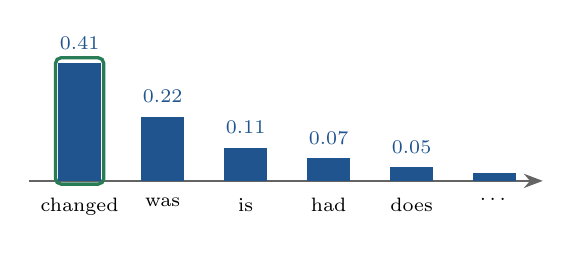
\begin{tikzpicture}[scale=0.68]
    \draw[ar] (0,0) -- (9.6,0);
    \foreach \i/\t/\h/\p in {0/changed/2.2/0.41, 1/was/1.2/0.22,
                             2/is/0.62/0.11, 3/had/0.42/0.07,
                             4/does/0.26/0.05, 5/\dots/0.14/{}}{
      \fill[nnblue, visible on=<2->]
        (\i*1.55+0.55,0) rectangle (\i*1.55+1.35,\h);
      \node[font=\scriptsize, below=1mm, visible on=<2->]
        at (\i*1.55+0.95,0) {\t};
      \node[font=\scriptsize, text=nnblue, above=0.5mm, visible on=<2->]
        at (\i*1.55+0.95,\h) {\p};
    }
    \draw[nngreen, very thick, rounded corners=2pt, visible on=<3->]
      (0.5,-0.06) rectangle (1.4,2.3);
  \end{tikzpicture}
  \end{center}
  \vspace{2mm}
  \begin{columns}[T,onlytextwidth]
    \begin{column}{0.478\textwidth}
      \begin{exampleblock}<4->{The loop}
        \small Pick one $\rightarrow$ append it $\rightarrow$ feed it all back
        in $\rightarrow$ repeat.
      \end{exampleblock}
    \end{column}
    \begin{column}{0.478\textwidth}
      \begin{alertblock}<5->{Worth internalising}
        \small No lookup. No notion of truth. Just a \textbf{plausible next
        token}.
      \end{alertblock}
    \end{column}
  \end{columns}
\end{frame}

%============================================================== 10
\begin{frame}{The journey, in one slide}
  \begin{columns}[T,onlytextwidth]
    \begin{column}{0.478\textwidth}
      \begin{block}{}
        \small
        \textbf{Neuron} --- a thing that holds a number.
        \medskip

        \onslide<2->
        \textbf{Weights \& biases} --- connection strength and firing
        threshold. The knobs.
        \medskip

        \onslide<3->
        \textbf{Gradient descent} --- score how wrong you are, then step
        downhill. Repeat.
      \end{block}
    \end{column}
    \begin{column}{0.478\textwidth}
      \begin{block}<4->{}
        \small
        \textbf{Embedding} --- a word as a point in space, where direction
        carries meaning.
        \medskip

        \onslide<5->
        \textbf{Attention} --- vectors look around and absorb context from
        their neighbours.
        \medskip

        \onslide<6->
        \textbf{LLM} --- all of the above, scaled, predicting one token at a
        time.
      \end{block}
    \end{column}
  \end{columns}
  \medskip
  \begin{exampleblock}<7->{}
    \centering
    Pixels lighting up $\rightarrow$ vectors moving through meaning.
    Same machine, bigger.
  \end{exampleblock}
\end{frame}

%============================================================== 11
\begin{frame}[plain]
  \transfade
  \vfill
  \centering
  {\Huge\bfseries\color{nnblue} Thank you}
  \vskip 8mm
  {\large Questions?}
  \vskip 12mm
  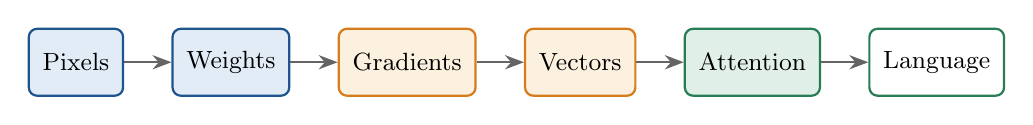
\begin{tikzpicture}[node distance=6mm]
    \node[box, visible on=<2->]              (p) {Pixels};
    \node[box, right=of p, visible on=<3->]  (w) {Weights};
    \node[obox, right=of w, visible on=<4->] (g) {Gradients};
    \node[obox, right=of g, visible on=<5->] (v) {Vectors};
    \node[gbox, right=of v, visible on=<6->] (a) {Attention};
    \node[gbox, right=of a, fill=white, visible on=<7->] (l) {Language};
    \draw[ar, visible on=<3->] (p) -- (w);
    \draw[ar, visible on=<4->] (w) -- (g);
    \draw[ar, visible on=<5->] (g) -- (v);
    \draw[ar, visible on=<6->] (v) -- (a);
    \draw[ar, visible on=<7->] (a) -- (l);
  \end{tikzpicture}
  \vfill
\end{frame}

\end{document}
